\section{Introduction}
\label{sec:introduction}

% state the learning objective 
The objective of this laboratory assignment is to study a circuit containing both independent and 
linearly dependent voltage and current sources. The circuit also contains 7 resistors, totaling 11 components conected both in series and in paralel.
The circuit has 7 nodes and 4 meshes. 
The circuit can be seen in Figure~\ref{fig:circuit_t1}.
The values of the resistors, the independent sources and the and the constants for the dependent 
sources are presented in figure .......********************. These values were obtained using the
Python script provided by the professor responsable for the laboratory assigment
and using 95815 as the seed 
%in series. The circuit can be seen if Figure~\ref{fig:circuit_t1}.

In Section~\ref{sec:analysis}, a theoretical analysis of the circuit is
presented. In Section~\ref{sec:simulation}, the circuit is analysed by
simulation, and the results are compared to the theoretical results obtained in
Section~\ref{sec:analysis}. The conclusions of this study are outlined in
Section~\ref{sec:conclusion}.

\begin{figure}[h] \centering
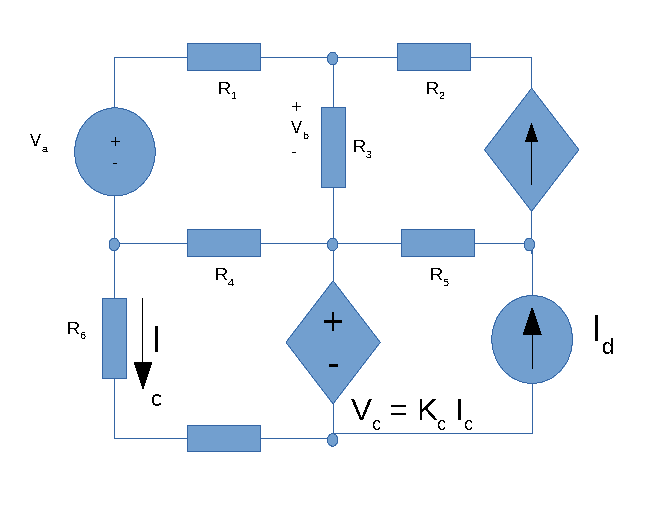
\includegraphics[width=0.4\linewidth]{circuit_t1.pdf}
\caption{Circuit in study}
\label{fig:circuit_t1}
\end{figure}

